\authorsetals work is done entirely in the complex plane.  In this section we review the complex numbers and some topological concepts of the complex plane.  Most definitions and theorems are borrowed from \textit{Fundamentals of Complex Analysis} by Saff and Snider \cite{Saff}.

If we picture the real numbers $\mathbb{R}$ as a one-dimensional number line, the set of complex numbers $\mathbb{C}$ can be thought of as a plane with $\mathbb{R}$ as its x-axis and the set of imaginary numbers as its y-axis.  Then, an element of $\mathbb{C}$  consists of both a real part and an imaginary part.

\begin{defn}
A \textbf{complex number} is an expression of the form $a + bi$ where $a, b \in \mathbb{R}$, and $i$ is defined as the imaginary number $\sqrt{-1}$.  Two complex numbers $a+bi$ and $c+di$ are said to be equal if and only if $a=c$ and $b=d$.
\end{defn}

So, for a complex number $z = a + bi$, $a$ is said to be the real part (denoted Re $z$) and $b$ is the imaginary part (denoted Im $z$).  With this notation we can write $z = \textrm{Re }z + i \textrm{ Im }z$.  Note that if $b=0$, then $z$ is a real number, while if $a=0$, then $z$ is a pure imaginary number.

Recall that the complex plane $\mathbb{C}$ can be combined with a distance function $d$:
\[d(z,w) = |z-w|\] where $z,w \in \mathbb{C}$ and $|z|$ is the modulus of $z$ defined as below.  Furthermore, this metric is induced by the usual norm of $\mathbb{C}$: $||z|| = \sqrt{x^2 + y^2}$ where $z = x+iy$ for $x,y \in \mathbb{R}$.  From this point on, this metric will be implied when we refer to $\mathbb{C}$ .

\begin{defn}
The \textbf{modulus} or (\textbf{absolute value}) of a number $z = a + bi$ is denoted $|z|$ and is given by
\[|z| := \sqrt{a^2 + b^2}\]
\end{defn}

Note that $|z|$ is always a nonnegative real number, and the only complex number whose modulus is zero is the number 0 itself.

The reflection of a point $z=a+bi$ across the real axis is the point $a-bi$.  The relationship between a number and its reflection plays a large role in complex analysis.

\begin{defn}
The \textbf{complex conjugate} of a number $z=a+bi$ is denoted $\conj{z}$ and is given by
\[\conj{z} := a-bi.\]
\end{defn}

The conjugate is important due to the numerous properties regarding the possible interactions between a complex number and its conjugate.

\begin{example}
First, it is clear that $z=\conj{z}$ if and only if $z$ is a real number.  Furthermore, the conjugate of the sum/difference of two complex numbers is equal to the sum/difference of their conjugates.  That is,
\[\overbar{z_1 + z_2} = \overbar{z_1} + \overbar{z_2}, \;\; \overbar{z_1 - z_2} = \overbar{z_1} - \overbar{z_2}.\]
Beyond these two properties are a number of other ones as well:
\begin{itemize}
\item $\overbar{(z_1z_2)} = \overbar{z_1}\,\overbar{z_2}$\\
Indeed, if $z_1 = a+bi$ and $z_2 = c+di$, then
\vspace{-1em}
\begin{align*}
\overbar{z_1z_2} &= \overbar{ac - bd + (ad + bc)i}\\
&= ac - bd - (ad + bc)i\\
&= ac - bd - adi - bci\\
&= (a - bi)(c-di)\\
&= \overbar{z_1}\,\overbar{z_2}.
\end{align*}
\item In addition, the following can be seen:
\[\overbar{\biggl(\frac{z_1}{z_2}\biggr)} = \frac{\overbar{z_1}}{\overbar{z_2}}, \; (z_2 \neq 0);\]
\[\textrm{Re } z = \frac{z+\overbar{z}}{2};\]
\[\textrm{Im } z = \frac{z-\overbar{z}}{2i}.\]
The last two properties demonstrate that the sum of a number and its conjugate is real, and the difference is imaginary, respectively.
\item The conjugate of a conjugate is, of course, the original number:
\[\overbar{(\overbar{z})} = z.\]
The final two properties are specifically used in \authorsetals paper:
\[|z| = |\overbar{z}|, \;\; z\overbar{z} = |z|^2.\]
The first of these is easy to see geometrically (Figure 1).

\begin{figure}[h]
\centering
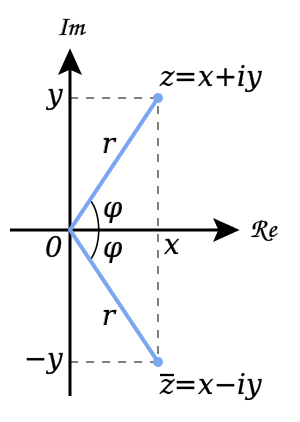
\includegraphics[scale=0.4]{images/complexmod.png}
\caption{Complex number and its modulus\cite{modulusimage}}
\end{figure}

The second can be proved easily:
\[z\overbar{z} = (a+bi)(a-bi) = a^2 + b^2 = |z|^2.\]
\end{itemize}
\end{example}

For functions of a real variable, we typically work with functions defined on an \textit{interval}, but this concept does not work for $\mathbb{C}$.  We must instead define some topological concepts for $\mathbb{C}$.

\begin{defn}
The \textbf{open disk} or \textbf{circular neighborhood} of a point $z_0$ is the set of all points $z$ which satisfy the inequality
\[|z-z_0| < p,\]
where $p$ is a positive real number.  This set consists of every point that lies inside the circle of radius $p$ around the center $z_0$.
\end{defn}

\begin{example}
The solution sets of the inequalities
\[|z-2| < 5, \;\;\; |z+i| < \frac{1}{2}, \;\;\; |z| < 8\]
are open disks centered at $2$, $-i$, and $0$ respectively.
\end{example}

A frequently used neighborhood is the \textit{open unit disk}:

\begin{defn}
The \textbf{open unit disk}, denoted $\mathbb{D}$ is as follows:
\[\mathbb{D} := \{z : |z| < 1\}.\]
\end{defn}

We will now define several closely related topological terms regarding sets.  We start with two terms in a single definition --- a two-for-one special, if you will.
\begin{defn}
For any set $S$, a point $z_0$ is called an \textbf{interior point} of $S$ if there is some open disk centered at $z_0$ which is completely contained in $S$.  If every point in $S$ is an interior point of $S$, we describe $S$ as an \textbf{open set}. 
\end{defn}

\begin{defn}
An open set $S$ is said to be \textbf{connected} if every pair of points can be joined by a curve which does not leave the set.  Alternatively, $S$ is connected if for all $p,q \in S$ there exists a finite collection of line segments contained in $S$ which join $p$ and $q$
\end{defn}

Essentially, a set is connected if it is a "single piece", geometrically speaking.  A \textit{convex set} is slightly more than this:

\begin{defn}
A set $S \in \mathbb{C}$ is said to be \textbf{convex} if
\[tp+(1-t)q \in S\]
for all $p,q \in S$ and for all $0 \leq t \leq 1$.  More simply, a set $S$ is convex if, for every pair of points in $S$, the line connecting the two points is contained within $S$.
\end{defn}

Note that, intuitively, all convex sets are connected, but a connected set is not necessarily convex.  Figure 2 shows this with geometric representations of sets --- (a) is both convex and connected, (b) and (c) are connected but not convex, and (d) is neither connected nor convex.

\begin{figure}[h]
\centering

\includegraphics[scale=0.5]{images/convexvconnected.png}
\caption{Convex vs. Connected Sets}
\end{figure}

\begin{defn}
A point $z_0$ is said to be a \textbf{boundary point} of a set $S$ if every neighborhood of $z_0$ contains at least one point of $S$ and at least one point not in $S$.  Simply put, $z_0$ is a boundary point if it exists on the edge of the set.  The set of all boundary points is called the \textbf{boundary} of $S$, and we will denote this $\partial(S)$.
\end{defn}

\begin{defn}
A set $S$ is said to be \textbf{closed} if it contains all of its boundary points.  Equivalently, $S$ is closed if its complement $\mathbb{C} \ S$ is open.
\end{defn}

\begin{example}
Let $\overbar{\mathbb{D}} = \{z : |z| \leq 1\}$.  This is a closed set, as it contains its boundary $\partial(\mathbb{D}) = \{z : |z| = 1\}$.  $\overbar{\mathbb{D}}$ is known as the \textit{closure of $\mathbb{D}$} or the \textit{closed unit disk}.
\end{example}

The final topological concepts we need for $\mathbb{C}$ are those of \textit{boundedness} and \textit{compactness}.

\begin{defn}
A set of points $S$ is said to be \textbf{bounded} if there exists some $r \in \mathbb{R}^+$ such that $|z| < r$ for every $z$ in $S$.  Equivalently, $S$ is bounded if it is contained in any neighborhood of the origin.  $S$ is \textbf{unbounded} if it is not bounded.
\end{defn}

\begin{defn}
A set that is both closed and bounded is said to be \textbf{compact}.
\end{defn}

We have sufficiently described the complex space $\mathbb{C}$ as an extension of the real numbers.  Furthermore, we have outlined a number of topological concepts for $\mathbb{C}$.  Later on, in the section on Conformal Mappings, we explore concepts from complex analysis much deeper --- specifically, we will describe analytic functions of the complex variable from a geometric standpoint.